%%%%%%%%%%%%%%%%%%%%%%%%%%%%%%%%%%%%%%%%%%%%%%%%%%%%%%%%%%%%%%%%%%%%%%%%
%                                                                      %
%     File: Thesis_Background.tex                                      %
%     Tex Master: Thesis.tex                                           %
%                                                                      %
%     Author: Andre C. Marta                                           %
%     Last modified :  4 Mar 2024                                      %
%                                                                      %
%%%%%%%%%%%%%%%%%%%%%%%%%%%%%%%%%%%%%%%%%%%%%%%%%%%%%%%%%%%%%%%%%%%%%%%%

\chapter{Background}
\label{chapter:background}

Insert your chapter material here.


%%%%%%%%%%%%%%%%%%%%%%%%%%%%%%%%%%%%%%%%%%%%%%%%%%%%%%%%%%%%%%%%%%%%%%%%
\section{Theoretical Overview}
\label{section:theory}

\textcolor{blue}{Modelo de baixa fidelidade, porque nao CFD}

%%%%%%%%%%%%%%%%%%%%%%%%%%%%%%%%%%%%%%%%%%%%%%%%%%%%%%%%%%%%%%%%%%%%%%%%
\section{Vehicle Dynamics}
\label{section:vehicle_dynamics}

\begin{equation}
    \mathbf{F} = \frac{\mathrm{d}}{\mathrm{d}t} \left( m \mathbf{V} \right)^E = \frac{\mathrm{d}}{\mathrm{d}t} \left( m \mathbf{V} \right)^V + \boldsymbol{\Omega} \times \left( m \mathbf{V} \right)^V
    \label{eq:force_equation}
\end{equation}


\begin{equation}
    \mathbf{M} = \frac{\mathrm{d}}{\mathrm{d}t} \left( \left[\mathbf{I}\right] \boldsymbol{\Omega} \right)^E = \frac{\mathrm{d}}{\mathrm{d}t} \left( \left[\mathbf{I}\right] \boldsymbol{\Omega} \right)^V + \boldsymbol{\Omega} \times \left( \left[\mathbf{I}\right] \boldsymbol{\Omega} \right)^V
    \label{eq:momentum_equation}
\end{equation}


\subsection{Inertia Tensor}


The angular momentum is to angular velocity what linear momentum is to linear velocity. Just as mass quantifies the resistance of an object to changes in its position, the inertia tensor, $\left[\mathbf{I}\right]$, measures an object's resistance to changes in its rotational motion. Mathematically, the inertia tensor, $\left[\mathbf{I}\right]$, is a symmetric 3 by 3 matrix 

\begin{equation}
    \left[\mathbf{I}\right]=\left[\begin{array}{c c c}{{I_{x x}}}&{{I_{x y}}}&{{I_{x z}}}\\ {{I_{x y}}}&{{I_{y y}}}&{{I_{y z}}}\\ {{I_{x z}}}&{{I_{y z}}}&{{I_{z z}}}\end{array}\right]
\end{equation}

where the matrix elements are the moments of inertia, about a reference frame $O_{xyz}$, computed as equations \ref{eq:ele_tensor_inertia1} and \ref{eq:ele_tensor_inertia2}

\begin{equation}
    I_{xx} = \smallint  \left( y^2 + z^2 \right) \mathrm{d}m \quad \text{and} \quad I_{yy} = \smallint  \left( x^2 + z^2 \right) \mathrm{d}m \quad \text{and} \quad I_{zz} = \smallint  \left( x^2 + y^2 \right) \mathrm{d}m
    \label{eq:ele_tensor_inertia1}
\end{equation}


\begin{equation}
    I_{xy} = \smallint  xy \, \mathrm{d}m \quad \text{and} \quad I_{xz} = \smallint  xz \, \mathrm{d}m \quad \text{and} \quad I_{yz} = \smallint  yz \, \mathrm{d}m
    \label{eq:ele_tensor_inertia2}
\end{equation}

In this study, the system is considered as a point mass and a rotor which means that only the rotor's mass is accounted into the inertia tensor. The rotor is composed by $N_b$ blades and each blade ha $m_b$ mass, which, by simplification, are considered as thin-plates for the inertia tensor calculation. In its principal axes centered in blade's center of mass, a thin-plate with its longer side along $y$-axes (meaning the blade span, $S_b$), its shorter side along $x$-axis (meaning the airfoil chord, $c_a$) and its thickness along $z$-axis (meaning the airfoil thickness, $t_a$). The inertia tensor of a flate plate in its principal axes is computed as in equation \ref{eq:inertia_tensor_principalaxes}

\begin{figure}[!htb]
    \centering
    \includegraphics[width=10cm]{Figures/background/inertia/inertia_scheme.png}
    \caption{Thin-plate position according to the principal axes ($O'$) inside the rotor' and blade's coordinate system, $O^r$ and $O^b$, respectively.}
    \label{fig:Inertia}
\end{figure}

\begin{equation}
    \left[\mathbf{I}\right]' = 
    \begin{bmatrix}
        \frac{1}{12}m_b(S_b^2+t_a^2) & 0 & 0\\
        0 & \frac{1}{12}m_b(c_a^2+t_a^2) & 0\\
        0 & 0 & \frac{1}{12}m_b(S_b^2+c_a^2)\\
    \end{bmatrix}
    \label{eq:inertia_tensor_principalaxes}
\end{equation}

For a rotor with multiple blades with a root distance from the blade to the rotor center, a transformation process must be introduced. Defining $\psi$ as the set azimutal position, the blades separated by an angle of

\begin{equation}
    \delta\psi = \frac{2\pi}{N_b}
\end{equation}

and, considering one of the blade's reference frame aligned with rotor's referece frame, introducing the rotation matrix along $z$-axis and considering the parallel axis theorem the total inertia frame of the rotor in rotor frame is

\begin{equation}
    \left[\mathbf{I}\right]^r = \sum_{m=1}^{N_b} \boldsymbol{R}_n^*\left[(m-1)\delta\psi\right] \left\{ \left[\mathbf{I}\right]' + m_b \epsilon^2 \boldsymbol{I} \right\} \boldsymbol{R}_n^*\left[(m-1)\delta\psi\right]^T
\end{equation}




%%%%%%%%%%%%%%%%%%%%%%%%%%%%%%%%%%%%%%%%%%%%%%%%%%%%%%%%%%%%%%%%%%%%%%%%

\section{Blade Element Theory}
\label{section:bet}

\begin{figure}[!htb]
    \centering
    \includegraphics[width=10cm]{Figures/background/bet/blade.png}
    \caption{\gls{bet} model with an highlight blade element in red. The blade reference frame (in blue) and the element reference frame (in green) are shown. Also the $n$-element velocity vector $\mathbf{U}^e_n$ in element reference frame is shown.}
    \label{fig:blade_bet}
\end{figure}

The Blade Element Theory (BET) is a simplefied modern model to study the rotor performance \cite{leishman_principles_2006}. With \gls{bet}, it is possible to make predictions about radiaL and azimuthal aerodynamic load distributions over the rotor disk. Its principel is based in a quasi-2D airfoils blade section which generate the aerodynamic forces and moments that shall be integrated over the blade length. With \gls{bet} methodology is possible to performe a rotor's first designing shape stage in terms of blade geometry.

Figure \ref{fig:blade_bet} presents the basic idea for the \gls{bet} in which it is possible a blade element $n$ (in red) with a width $\mathrm{d}y$ at a a distance $y$ from the blade root. The element is considered as a 2D airfoil under a flow with a velocity $\mathbf{U}_n$.

For each blade element, the general flow and forces applied and the pressure center of the airfoil are presented in figure \ref{fig:element_bet}. All over the blade and azimutal postions this is not a standard configuration for the reference frames, forces and velocities. This influences the way that angles are determined in each element. This is taken into considerantion and the following equations are for all the cases different.


\begin{figure}[!htb]
    \centering
    \includegraphics[width=9cm]{Figures/background/bet/element.png}
    \caption{Blade element with flow enviroment and forces aplied.}
    \label{fig:element_bet}
\end{figure}




The aerodynamic loads, in the aerodynamic reference frame, $O^a$, are also represented in figure by \ref{fig:element_bet}, where its horizonal compenent (in $X^a$ axis) or drag force, $\mathrm{d}D_n^a$, is computed as

\begin{equation}
    \mathrm{d}D^a_n = \frac{1}{2} \rho c ||\mathbf{U}^a_n||^2 C_d,
    \label{eq:drag_element}
\end{equation}

while vertical compenent (in $Z^a$ axis) or lift force is computed as

\begin{equation}
    \mathrm{d}L^a_n = \frac{1}{2} \rho c ||\mathbf{U}^a_n||^2 C_l,
    \label{eq:lift_element}
\end{equation}

where $\rho$ is air density, in \unit{\kg\per\meter^3}, $c$ is the airfoil cord in \unit{\meter} and $C_l$ and $C_l$ are the lift and drag coefficients, respectively, as functions of the angle of attack, $\alpha$, and number of Reynolds, $Re$,

\begin{equation}
    Re = \frac{\rho ||\mathbf{U}^a_n|| c}{\mu}
    \label{eq:reynolds_number}
\end{equation}

where $\mu$ is the dynamic viscosity of the air, meaning that

\begin{equation}
    C_l \equiv C_l(\alpha, Re) \quad \text{and} \quad C_d\equiv C_d(\alpha, Re).
\end{equation}

In section \ref{section:aero_model}, a detailed explanation on how the lift, $C_l$, and drag, $C_d$ coefficients are obtained is presented. Keeping focus on the aerodynamic load, it is possible to construct the elementary aerodynamic force in the aerodynamic reference frame as

\begin{equation}
    d\mathbf{F}^a_n = \begin{bmatrix}
        \mathrm{d}D^a_n \\ 0 \\ \mathrm{d}L^a_n
    \end{bmatrix}
    \label{eq:vector_aero_force}
\end{equation}

In the other words, vector presented in \ref{eq:vector_aero_force} is the force vector of each that shall be writen in Earth-fixed coordinades for equation force equation \ref{eq:force_equation}. For a simpler approach, the choice stands for computing the aerodynamic referece frame forces, denoted with upscript $^a$, and apply a cicle to compute the rotor's total force , $\mathbf{F}^r_{rotor}$, as as function of all the elementary forces, $\mathrm{d}\mathbf{F}^a_n$, along the blade length and azimutal positions. then, its necessary to introduce the rotation matrices between the various reference frames. First from the aerodynamic to element frame, then to blade frame and rotor frame, and final to the Earth-fixed frame. A the blade and the element reference frames are only translated being with the same orientation which means that the rotation matrix between the blade and element reference frames is the identity matrix, $\mathbf{I}$. So equation \ref{eq:aero_to_blade_force} presents the direct transformation of the elementary aerodynamic force, $d\mathbf{F}^a$, from the aerodynamic reference frame to the blade reference frame.

\begin{equation}
    d\mathbf{F}^b = \boldsymbol{R}^{ot}(\hat{y}, \phi_n) d\mathbf{F}^a
    \label{eq:aero_to_blade_force}
\end{equation}

$\boldsymbol{R}^{ot}(\hat{y}, \phi_n)$ states for the rotation matrix along $y$-axis and the inflow angle for each of the the blade's elemetns, $\phi_n$. The rotation process is described in section \ref{section:rotation_matrices}. Finally in the rotor reference frame, the elementary force, $d\mathbf{F}^r$, is given by the rotation given by the blades ' azimuthal angle, $\psi_n$, as

\begin{equation}
    d\mathbf{F}^r_n = \boldsymbol{R}^{ot}(\hat{z}, \psi_n) d\mathbf{F}^b
\end{equation}

or as a sequence of both rotations, $\phi_n$ and $\psi_m$,

\begin{equation}
    d\mathbf{F}^r_n = \boldsymbol{R}^{ot}(\hat{z}, \psi_m) \boldsymbol{R}^{ot}(\hat{y}, \phi_n) d\mathbf{F}^a.
    \label{eq:element_force_rotor_frame}
\end{equation}

In terms of applied torque from the aerodynamic forces to the rotor's center, the elementary torque applied for each element, $d\mathbf{Q}^r_n$, is given by 

\begin{equation}
    d\mathbf{Q}^r_n = \mathbf{r}^r_n \times \left[ \boldsymbol{R}^{ot}(\hat{z}, \psi_m) \boldsymbol{R}^{ot}(\hat{y}, \phi_n) d\mathbf{F}^a \right] 
    \label{eq:element_torque_rotor_frame}
\end{equation}

where $\mathbf{r}^r_n$ stand for the force arm from the rotor's center to the blade element. As a simplification of the next formulas, equation  \ref{eq:simplication_rotation_bet} is introduced

\begin{equation}
    \boldsymbol{R}^{ot}(\hat{z}, \psi_m) \boldsymbol{R}^{ot}(\hat{y}, \phi_n) \equiv \underset{a \to r}{\boldsymbol{R}^{ot}}\
    \label{eq:simplication_rotation_bet}
\end{equation}

and then, force expression, \ref{eq:element_force_rotor_frame}, can be rewritten as

\begin{equation}
    d\mathbf{F}^r_n = \underset{a \to r}{\boldsymbol{R}^{ot}} d\mathbf{F}^a.
    \label{eq:element_force_rotor_frame_simplified}
\end{equation}

and for the torque, \ref{eq:element_torque_rotor_frame}, the same expression can be used

\begin{equation}
    d\mathbf{Q}^r_n = \mathbf{r}^r_n \times \left[ \underset{a \to r}{\boldsymbol{R}^{ot}}  d\mathbf{F}^a \right] 
    \label{eq:element_torque_rotor_frame_simplified}
\end{equation}.

Knowing all the elementary forces and torques, the total force and torque applied to the rotor can be computed by integrating over the blade length between the blade's root, at a distance $\epsilon$, and the blade's tip, at a distance of $\epsilon + L$. For the the $m$-blade's force is given by

\begin{equation}
    \mathbf{F}^r_{m} = \int_\epsilon^{L+\epsilon} d\mathbf{F}^r_n \mathrm{d}y = \int_\epsilon^{L+\epsilon} \underset{a \to r}{\boldsymbol{R}^{ot}}  d\mathbf{F}^a \mathrm{d}y
\end{equation}


while blade's torque is computed as

\begin{equation}
    \mathbf{Q}^r_{m} = \int_\epsilon^{L+\epsilon} d\mathbf{Q}^r_n  \mathrm{d}y = \int_\epsilon^{L+\epsilon} \mathbf{r} \times \left[ \underset{a \to r}{\boldsymbol{R}^{ot}}  d\mathbf{F}^a \right] \mathrm{d}y
\end{equation}

As a final step, the forces shall be integrated as a function of the rotor's azimutal discretization, $\psi_m$. To achieve this the integration is assumed as as aritemetic mean of all of the forces and torques producec for the blade in each of the azimutal sections

\begin{equation}
    \mathbf{F}_{rotor}^r = \frac{N_b }{N_{\psi}} \sum_{m=1}^{N_{\psi}} \mathbf{F}^r_{m} = \frac{N_b }{N_{\psi}} \sum_{m=1}^{N_{\psi}} \int_\epsilon^{L+\epsilon} \underset{a \to r}{\boldsymbol{R}^{ot}}  d\mathbf{F}^a \mathrm{d}y
    \label{eq:total_rotor_force_rotor_frame}
\end{equation}

\begin{equation}
    \mathbf{Q}_{rotor}^r = \frac{N_b }{N_{\psi}} \sum_{m=1}^{N_{\psi}} \mathbf{Q}^r_{m} = \frac{N_b }{N_{\psi}} \sum_{m=1}^{N_{\psi}} \int_\epsilon^{L+\epsilon} \mathbf{r} \times \left[ \underset{a \to r}{\boldsymbol{R}^{ot}}  d\mathbf{F}^a \right] \mathrm{d}y
    \label{eq:total_rotor_torque_rotor_frame}
\end{equation}

Also, in equations \ref{eq:total_rotor_force_rotor_frame} and \ref{eq:total_rotor_torque_rotor_frame}, it is intoduced the term of the number of blades, $N_b$, as the rotor is composed by multiple blades. $\mathbf{F}_{rotor}^r$ and $\mathbf{Q}_{rotor}^r$ expressions models the rotor's aerodynamic behaviour.


\subsection{ Pitch and Incidence Angle, Angle of Attack,}

When computing the aerodynamic forces and moments the angle of attack presents a crucial factor for the 2D aerodynamic lift and drag coefficients

\begin{figure}[!htb]
    \centering
    \includegraphics[width=5cm]{Figures/background/bet/phi_angle.png}
    \caption{Blade element with flow enviroment and forces aplied.}
    \label{fig:phi_angle}
\end{figure}



The velocity component in each blade element, $\mathrm{U}_n$, depends on its radial position due to the rotation motion of the blade - this component is deeply analyzed further in section \ref{section:element_velocity}. The angle between the velocity vector and the horizontal plane of the rotor is called the inflow angle, $\phi$. To compute the inflow angle, $\phi$, one can introduce an auxiliar unitary vector, $\mathrm{e}^e_x = \begin{bmatrix} 1 & 0 & 0 \end{bmatrix}$ aligned with the $X^e$ axis, and writting the velocity vector in element reference frame, $\mathrm{U}_n^e$, the cosine of the inflow angle and the unitary vector is given by equation \ref{eq:cosine_inflow}



\begin{equation}
    \cos \phi = \frac{\mathbf{U}_n^e \cdot \mathbf{e}^e_x}{||\mathbf{U}_n^e|| \cdot ||\mathbf{e}_x^e||} \implies \phi = \cos^{-1} \left( \frac{\mathbf{U}_n^e|_x}{||\mathbf{U}_n^e||}\right)
    \label{eq:cosine_inflow}
\end{equation}

where $\mathbf{U}_n^e|_x$ is the $x$-component of the velocity vector in element reference frame. The equation \ref{eq:cosine_inflow} does not take into consideration both the $\mathbf{U}_n$ if it is upwards or downwards in termns of the $U_P$ component. As seen in figure \ref{fig:element_bet}, the inflow angle, $\phi$, is negative but when \ref{eq:cosine_inflow} is used , the angle is positive. For changing this equation \ref{eq:cosine_inflow_corrected} is introduced.

\begin{equation}
    \begin{cases}
        \phi = \cos^{-1} \left( \frac{\mathbf{U}_n^e|_x}{||\mathbf{U}_n^e||}\right), \text{ if } U_P <= 0\\
        \phi = - \cos^{-1} \left( \frac{\mathbf{U}_n^e|_x}{||\mathbf{U}_n^e||}\right), \text{ if } U_P > 0
    \end{cases}
    \label{eq:cosine_inflow_corrected}
\end{equation}

The angle between the airfoil chordline and the horizonal plane of the rotor is called the pitch angle denoted as $\theta$ in figure \ref{fig:element_bet}. The pitch angle, $\theta$, can be defined as collective or cyclic pitch angle. All of the blade components along the rotor blade have the same collective pitch angle, which means that the pitch changes uniformly throughout the blade. Usually, the pilot regulates this to change the total lift the rotor produces. However, when the rotor rotates, the cyclic pitch angle changes for various blade parts. By controlling the rotor disc's orientation, this variation enables the aircraft to tilt in a certain direction. Asymmetrical lift distribution and directional control are made possible by the cyclic pitch adjustment, which modifies the blade's angle of attack based on its azimuth location. For the present study, the pitch angle is set for each of the blade's element and is the same distribution for all the blades that compose the rotor and does not change over time. 

The angle of attack, denoted as $\alpha$, is the angle between the airfoil chord line and the relative airflow experienced by the blade element. It is a crucial parameter in determining the aerodynamic forces acting on the blade. The angle of attack depends on both the pitch angle,  $\theta$, and the inflow angle, $\phi$, which include the induced velocity generated by the rotor and the forward motion of the aircraft. 

To determine the angle of attack considering all pitch angle, $\theta$, and inflow angles, $\phi$, over the blade length and azimultal distribution, equation 

\begin{equation}
    \begin{cases}
        \alpha = \theta - \phi \text{ if } \theta < \phi\\
        \alpha = \phi - \theta \text{ if } \phi < \theta\\
    \end{cases}
    \label{eq:angle_of_attack}
\end{equation}

\subsection{The Element's Velocity}
\label{section:element_velocity}


\begin{equation}
    \left(\mathbf{U}_\infty\right)^e_n = \mathbf{V}^e_{vehicle} + \mathbf{r}_n^e \times \boldsymbol{\Omega}_{vehicle}^e + \mathbf{r}_n^e \times \boldsymbol{\Omega}_{rotor}^e + \mathbf{V}_{wind}^e + \mathbf{V}_{induced}^e
\end{equation}


\section{Rotation matrices}
\label{section:rotation_matrices}

Considering any inertial reference frame $O(\hat{x},\hat{y},\hat{z})$ and a rotated reference frame $O'(\hat{x}',\hat{y}',\hat{z}')$, the Euler angles, $\Xi$ that the define the rotation of $O'$ related to $O$ is presented in figure \ref{fig:rotation_frames_img}

\begin{figure}[!htb]
    \centering
    \includegraphics[width=6cm]{Figures/background/rotation_matrices/rotation_frames.png}
    \caption{Reference frame rotation Euler angles, adapted from \cite{schwab_how_2006}}
    \label{fig:rotation_frames_img}
\end{figure}

The following expressions, presented in equations \ref{eq:rotatio_zz}, \ref{eq:rotatio_yy} and \ref{eq:rotatio_xx}, define the rotation matrices of a rotation over the each of the reference axis $\hat{Z}$, $\hat{Y}$ and $\hat{X}-$axis. For the rotation matrices, it is used a simplified nomenclature where $c_{\delta_{*}}$ are $s_{\delta_{*}}$ are cosine and sine functions of the angle $\delta_{*}$. The total rotation matrix, considering the Tailt-Bryan Convention is

\begin{equation}
    {R o t({\hat{z}},\delta_1)}={\left[\begin{array}{l l l}{1}&{0}&{0}\\ {0}&{c_{\delta_1}}&{-s_{\delta_1}}\\ {0}&{s_{\delta_1}}&{c_{\delta_1}}\end{array}\right]}
    \label{eq:rotatio_zz}
\end{equation}

\begin{equation}
    Rot(\hat{y},\delta_2)=\left[\begin{array}{c c c}{{c_{\delta_2}}}&{{0}}&{{s_{\delta_2}}}\\ {{0}}&{{1}}&{{0}}\\ {{-s_{\delta_2}}}&{{0}}&{{c_{\delta_2}}}\end{array}\right]
    \label{eq:rotatio_yy}
\end{equation}

\begin{equation}
    Rot({\hat{x}},{\delta_3})={\left[\begin{array}{l l l}{{{c}_{\delta_3}}}&{{-{s}_{\delta_3}}}&{{0}}\\ {{{s}_{\delta_3}}}&{{{c}_{\delta_3}}}&{{0}}\\ {{0}}&{{0}}&{{1}}\end{array}\right]}
        \label{eq:rotatio_xx} 
\end{equation}


After defining expressions \ref{eq:rotatio_zz}, \ref{eq:rotatio_yy} and \ref{eq:rotatio_xx}, the rotation matrix between the aerodynamic reference frame adn the rotor reference frame can be computed as

\begin{equation}
    \boldsymbol{R}^{ot}_{a \to r} = \boldsymbol{R}^{ot}(\hat{z}, \psi_m) \boldsymbol{R}^{ot}(\hat{y}, \phi_n) =
    \begin{bmatrix}
    c_{\phi_n} & 0 & s_{\phi_n} \\
    s_{\psi_m}s_{\phi_n} & c_{\psi_m} & -s_{\psi_m}c_{\phi_n} \\
    -c_{\psi_m}s_{\phi_n} & s_{\psi_m} & c_{\psi_m}c_{\phi_n}
    \end{bmatrix}    
    \label{eq:rotatio_aero_rotor}
\end{equation}



%%%%%%%%%%%%%%%%%%%%%%%%%%%%%%%%%%%%%%%%%%%%%%%%%%%%%%%%%%%%%%%%%%%%%%%%

\section{2D Aerodynamic Model}
\label{section:aero_model}


\textcolor{blue}{Motivar a necessidade de haver um modelo aerodinâmico}

As seen in section \ref{section:bet}, the \gls{bet} is a based model, in short words, defined a sum of elementary 2D airfoil setions. Then its crucial for its implementation a computational method to obtain the drag, $C_d (\alpha, Re) $, and  lift, $C_l (\alpha, Re)$, coefficients for 2D airfoils, in equations \ref{eq:drag_element} and \ref{eq:lift_element}.

\textcolor{blue}{questões computacionais}

Also \gls{bet} has critical consideration rather the number of elements used to define a blade. The higher the number of elements and azimutal discretization, the higher the number of calculations needed to be perform a rotor analysis. This means that for a time-dependent model as a free-fall considered in this work, more critical it is, in term of computational time, to perform any simulation. So a fast model should be considered.

\textcolor{blue}{altos angulos de ataque}

For choosing a airfoil analysis, one must consider the rotor dynamics. In this study, the rotor is under the phenomena of autorotation which has its displacement mainly in descent direction, then some considerations should be made about the angles of attack. On blade's root, the angular velocity is smaller when compared to the blade's tip. Meaning, the inflow angle is mainly composed by a vertical component rather than a horizontal component. So, a wider range of angles of attack should be considered. Also, if it is considered a pure vertical descent mode and small rotor angular velocity, the angles of attack while certainly be near 90$^{\circ}$ meaning that the rotor will work on a stall model. A reference to the pitch angle, $\theta$, and the blade twist should be made, however for thin airfoils it is known that for angles near 20$\sim$30$^\circ$, depending on thickness and camber, the airfoils starts to operate as a flate plate on stall mode, with completely separate boundary layers.

So, in this sense, to lead with this problems NeuralFoil \cite{sharpe_neuralfoil_nodate} presents a simple solution under the Aerosandbox package \cite{sharpe_aerosandbox_nodate,sharpe_accelerating_nodate}. NeuralFoil is a neural-network based model for 2D airfoils, which is able to predict the drag and lift coefficients for a wide range of airfoils, Reynolds and Mach numbers, and angles of attack. This model is based on a set neural-networks pre-trained with XFOIL meaning that the model is able to predict the drag and lift coefficients inside the scope where XFOIL presents not only numeric convergency but also physical convergency. 

An output parameter from the NeuralFoil (and from any neural-network) is the confidence level of the ouput. These parameter is presented in figure figure \ref{fig:neuralfoil_confidence}, where the black region is the range where the model is able to predict the drag and lift coefficients with a confidence level of 95\%. 

\begin{figure}[!htb]
    \centering
    \includegraphics[width=8cm]{Figures/background/aero/NeuralFoil_Confidence_2D_black.png}
    \caption{NeuralFoil confidence level for NACA 0012 airfoil for Reyndols number from $10^3$ to $10^9$}
    \label{fig:neuralfoil_confidence}
\end{figure}

Analysing the figure \ref{fig:neuralfoil_confidence}, it is possible to state some key aspects of the NeuralFoil model:

\begin{enumerate}
    \item As expected NeuralFoil is limited to the angles of attack where XFOIL presents physical convergency - before the the stall angle where . This values presents a symmetric result due to the fact that airfoil is also symmetric (without camber).
    
    \item For the ultra low Reynolds, above $~ 10^3$, the model is not able to predict the drag and lift coefficients with a confidence level. In this Reynolds Number interval, the XFOIL is not able to predict the need coefficients once the flow is completely different. At $Re ~ 10^3$ there is an absence of separation bubble as  concluded by Alam er al. (2010) \cite{alam_ultra-low_2010}. Not having a separation bubble the flow keeps laminar for a long longitudinal distance delaying the transition, so no stall occurs, being the maximum coefficients determined at $\alpha \approx 45 ^{\circ}$
    
    \item At $Re = 10^5 \approx 10^6$, the stall angle varies creating over the Reynolds number interval, meaning it is important to make further consideration for the angles of attack after the stall occurs. After the the stall occurring XFOIL is not able to detemine the transient phenomena of the flow once it is build based on a panel methos which does not have capabilities to perform an airfoiol analysis with time-varient lift and drag coefficients.

\end{enumerate}


NeuralFoil \cite{sharpe_neuralfoil_nodate} is a fast and reliable model to predict the drag and lift coefficients for 2D airfoils inside the black region in figure \ref{fig:neuralfoil_confidence}, however there is a need to amplify the aerodynamic model with a certain good accuracy for the post-stall regime.


\textcolor{blue}{Definição do range de angulos de ataque e de números de reynolds}\\
\textcolor{blue}{Apresentação do AERODAS modelos aerodinâmico}\\
\textcolor{blue}{Explicar capacidades e deficiencias}\\
\textcolor{blue}{Apresentação do NeuralFoil e vantagens na utilização como base de dados para o AERODAS}\\
\textcolor{blue}{Drawbacks do neuralfoil – confiança da rede neuronal para os grandes angulos de ataque}\\
\textcolor{blue}{Definição do intervalo de confiança do neural foil}\\
\textcolor{blue}{Ligação com o AERODAS – NEURALFOIL}\\
\textcolor{blue}{Resultados para 2 perfis diferentes}\\


%%%%%%%%%%%%%%%%%%%%%%%%%%%%%%%%%%%%%%%%%%%%%%%%%%%%%%%%%%%%%%%%%%%%%%%%
\section{Atmosphere Model}
\label{section:atmosphere_model}

The 2D aerodynamic loads, drag $\mathrm{d}D^a_n$ and lift $\mathrm{d}D^a_n$, as expressed in equations \ref{eq:drag_element} and \ref{eq:lift_element}, are directly proportional to the air density, $\rho$. Also, the atmospheric proprieties during the descent flight change with altitude, including the dynamic viscosity, $\mu$, importante to compute the Reynolds number, in equation \ref{eq:reynolds_number}. In this sense, an atmospheric model is a crucial factor when computing aerodynamic loads, as it will directly impact the values of these loads. 

On the literature there are many atmospheric models such as the \gls{isa} \cite{noauthor_iso_nodate}, \gls{nasa}'s \gls{eam} \cite{noauthor_earth_nodate} and NRLMISES00 \cite{picone_nrlmsise00_2002}. All these options seemed a good choice, but to accomplish one of  this work goals accuracy-time commitment, a critical anaylsis is necessary.

Before the analysis, for the current application, \gls{isa} model is computed using MATLAB \cite{matlab_version_2024} Aerospace Toolbox \cite{noauthor_aerospace_nodate} function \textit{atmosisa} \cite{noauthor_atmosisa_nodate} and NRLMISES00 model is computed using provided function in MATLAB \cite{matlab_version_2024} Central File Exchange \cite{noauthor_atmosphere_2025}. For the \gls{eam} a MATLAB \cite{matlab_version_2024} code was created by the author. However , not all these models compute all necessary parameteres directly, namely the dynamic viscosity, $\mu$, which further used to compute Reynolds number, $Re$. Then it was introduced the Sutherland's Law to compute the dynamic viscosity

\begin{equation}
    \mu(T) = \mu_0 \left( \frac{T_0 + S}{T + S} \right) \left( \frac{T}{T_0} \right)^{3/2}.
\end{equation}

\noindent for models EAM \cite {noauthor_earth_nodate, noauthor_atmosisa_nodate} and NRLMISES00 \cite{picone_nrlmsise00_2002, noauthor_atmosphere_2025}.

Once all the necessary code for running the different atmospheric models is completed, figures \ref{fig:atmos_models_comp_temp} and \ref{fig:atmos_models_comp_density} present a comparison of temperature and density between the three models for altitudes ranging from 0 to 100 \unit{\km}, respectively. This range was chosen to provide a clearer view of the plots for the different models. However, it is important to note that the models are not valid for all altitudes. For instance, the \gls{isa} model is valid only between sea level and the mesopause (0 to approximately 85 \unit{\km}) and the NRLMISES00 model is valid up to 1000~\unit{\km}. With \gls{eam} the height is not at limited by the model, however it only showed good agreement with the other models up to 50 \unit{\km} for the temperature profile as it can be seen in figure \ref{fig:atmos_models_comp_temp}.


\begin{figure}[!htb]
	\centering
	\begin{minipage}{0.48\textwidth}
		\centering
		\includegraphics[width=\textwidth]{Figures/background/atmos/temperature_plot.png}
		\caption{Temperature Comparison}
		\label{fig:atmos_models_comp_temp}
	\end{minipage}
	\hfill
	\begin{minipage}{0.48\textwidth}
		\centering
		\includegraphics[width=\textwidth]{Figures/background/atmos/density_plot.png}
		\caption{Density Comparison}
		\label{fig:atmos_models_comp_density}
	\end{minipage}
\end{figure}

For the density profile, all the three models shwo a good agreement with minor a relative minor error between them. However, for the temperature profile, the analysis is not so straightforward. In the lower altitudes (up to 10 km), all models exhibit a roughly linear decrease in temperature, although NRLMSISE-00 shows slight irregularities. Between 10 and 20 km, \gls{isa} displays the characteristic plateau of the tropopause, while \gls{eam} and NRLMSISE-00 present smoother transitions. Above 20 km, significant differences become apparent: NRLMSISE-00 accurately captures the sharp temperature increase in the thermosphere, reflecting its detailed physical basis, whereas \gls{isa} maintains a simplified, smoothed profile, lacking this feature. \gls{eam} diverges from \gls{isa} but does not fully replicate the extreme rise observed in NRLMSISE-00. Overall, \gls{isa} serves as a practical but simplified model, NRLMSISE-00 provides higher accuracy at extreme altitudes, and \gls{eam} strikes a balance between simplicity and realism. This comparison underscores the distinct strengths and limitations of each model in representing atmospheric temperature variations.

Further anaylsis relevante to the atmospheric models performance is presented in table \ref{tab:atmos_model_speed}, Where the execution time of diferent number of functions calls are done. From this table, it is possible to understande that the NRLMISE00 model creates a huge impact when a simulation has a low descent ratio. This is because the NRLMISE00 model is more complex and computationally expensive than the other two.

\begin{table}[!htb]
    \centering
    \begin{tabular}{
    >{\columncolor[HTML]{FFFFFF}}l 
    >{\columncolor[HTML]{FFFFFF}}r
    >{\columncolor[HTML]{FFFFFF}}r
    >{\columncolor[HTML]{FFFFFF}}r }
    \hline
    {\color[HTML]{000000} No. Function Calls} & \multicolumn{1}{r}{\cellcolor[HTML]{FFFFFF}{\color[HTML]{000000} EAM \cite{noauthor_iso_nodate}}} & \multicolumn{1}{r}{\cellcolor[HTML]{FFFFFF}{\color[HTML]{000000} ISA \cite{noauthor_earth_nodate}}} & \multicolumn{1}{r}{\cellcolor[HTML]{FFFFFF}{\color[HTML]{000000} NRLMISES00 \cite{picone_nrlmsise00_2002}}} \\ \hline
    {\color[HTML]{000000} 1}                  & {\color[HTML]{000000} 0.8 \unit{\ms}}                                                                                           & {\color[HTML]{000000} 25.1 \unit{\ms}}                                                                                        & {\color[HTML]{000000} 46.6 \unit{\ms}}                                                                                                  \\
    {\color[HTML]{000000} 10}                 & {\color[HTML]{000000} 1.0 \unit{\ms}}                                                                                           & {\color[HTML]{000000} 5.1 \unit{\ms}}                                                                                           & {\color[HTML]{000000} 25.0 \unit{\ms}}                                                                                                 \\
    {\color[HTML]{000000} 100}                & {\color[HTML]{000000} 0.1 \unit{\ms}}                                                                                           & {\color[HTML]{000000} 19.1 \unit{\ms}}                                                                                          & {\color[HTML]{000000} 173.7 \unit{\ms}}                                                                                                \\
    {\color[HTML]{000000} 1000}               & {\color[HTML]{000000} 0.4 \unit{\ms}}                                                                                           & {\color[HTML]{000000} 173.9 \unit{\ms}}                                                                                         & {\color[HTML]{000000} 1.6 \unit{\s}}                                                                                                   \\
    {\color[HTML]{000000} 10000}              & {\color[HTML]{000000} 3.0 \unit{\ms}}                                                                                           & {\color[HTML]{000000} 1.3 \unit{\s}}                                                                                             & {\color[HTML]{000000} 21.0 \unit{\s}}                                                                                                  \\
    {\color[HTML]{000000} 100000}             & {\color[HTML]{000000} 28.1 \unit{\ms}}                                                                                          & {\color[HTML]{000000} 18.1 \unit{\s}}                                                                                           & {\color[HTML]{000000} 3.7 \unit{\minute}}                                                                                                 \\ \hline
    \end{tabular}
    \caption{Computational times for different number of function calls for the three atmospheric models.}
    \label{tab:atmos_model_speed}
\end{table} 

Taking into considerantion both profile and computational anaylis clearily theres some advantages of using all the models. \gls{eam} is quite accurate and fast for low altitudes, once \gls{isa} is in accordance to the others models for altitudes until 80 \unit{\km} and realtive fast, and finally the NRLMISE00 model is the slowest computationally but provides higher varitions in certain atmosphere regions. For the final implementation, the choice of the model considered in this work, \gls{isa} is the choosen model for all the analysis presented furter in this work, once it provides quite fast computational times and a wide range of altitudes, namely the range of the DAEDALUS \cite{riegler_daedalus_2018} project used in next section to validate the model.


\section{Prandtl Tip Losses Factor}

In the context of helicopter rotor or wind turbine rotor systems, an inherent challenge arises as the blades near the tips experience a higher velocity compared to those near the hub. This speed differential introduces complications such as increased drag, heightened turbulence, and the formation of tip vortices, spiral patterns of rotating air trailing behind the rotor blade tips \cite{leishman_principles_2006}. These tip vortices signify a notable source of energy loss, which contributes to a reduction in overall system efficiency. Over the years, various strategies have been studied to mitigate this tip loss, including optimising rotor blade shapes, adjusting blade twists, and incorporating advanced aerodynamic features.

Efforts to address tip loss also involve the application of the Prandtl tip loss function \cite{leishman_principles_2006, ramdin_prandtl_nodate}. Prandtl tip loss is the decrease in aerodynamic efficiency that propeller or rotor blades undergo as they get closer to their tips as a result of following vortices that are created as they go through the air. Overall efficiency is reduced as a result of this phenomenon. Within the field of aerodynamics, the Prandtl tip loss function is a mathematical instrument that is specifically utilised to model and quantify this phenomenon \cite{leishman_principles_2006}. Its main purpose is to take into account the induced velocity caused by the tip vortices and then modify the effective inflow velocity that the blade experiences at the tip.


In the book of professor Leishman \cite{leishman_principles_2006}, the Prandtl's Tip Loss function is addressed considering two different cases: 1) no tip losses at the rotor root; 2) tip losses in tip and root of the rotor. For the first case, function which estimates a lift variation is given by equation \ref{eq:tiplossprandtl},

\begin{equation}
    F = \frac{2}{\pi} \cos^{-1}\left(\exp{\left(-f\right)}\right)
    \label{eq:tiplossprandtl}
\end{equation}

\noindent where $f$ is a function of the geometric properties of the blade and the inflow angle $\phi = \frac{\lambda (r)}{r}$

\begin{equation}
    f_{tip} = \frac{N_b}{2} \left( \frac{1-r}{r\phi}\right)
\end{equation}

Applying the the factor $F$ to the lift distribution over the blade radius, the figure \ref{fig:prandtltiploss} presents how the function varies with the number of blades and the inflow angle over the radius of the blades. From the figure \ref{fig:prandtltiploss}, is possible to see that this function does not consider the tip loss in the rotor center, as the function is the maximum value in the beginning of the rotor.

\begin{figure}[!htb]
    \centering
    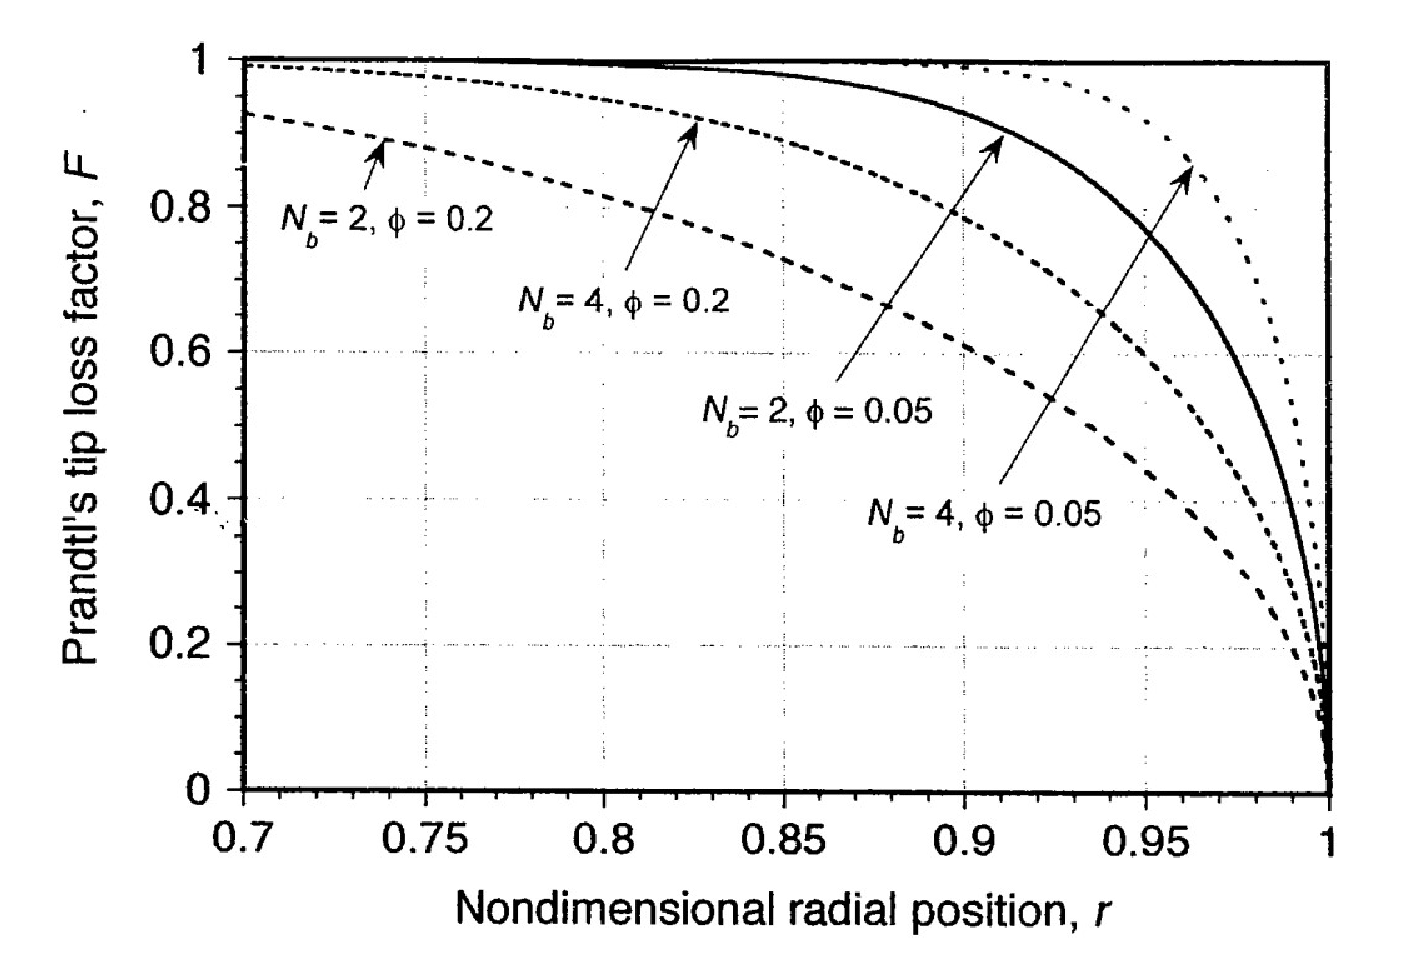
\includegraphics[width=0.5\textwidth]{Figures/background/tiplosses/prandtltiploss.eps}
    \caption[Prandtl Tip Loss function versus radial position for two- and four-bladed rotor]{Prandtl Tip Loss function versus radial position for two- and four-bladed rotor, from \cite{leishman_principles_2006}}
    \label{fig:prandtltiploss}
\end{figure}

However, this assumption is not physically correct and then the second option appears in \cite{leishman_principles_2006}. For considering the loss of tips at the root of the blade, the equation \ref{eq:tiplossesroot} is considered.

\begin{equation}
    f_{root} = \frac{N_b}{2} \left( \frac{r}{\left(1-r\right)\phi}\right)   
    \label{eq:tiplossesroot}
\end{equation}

For combining root and tip losses, the factor $f$ considered is the combinations of \ref{eq:tiplossprandtl} and \ref{eq:tiplossesroot}. The combination of root an d tip losses is presented in figure \ref{fig:fullprandtltiplossfunction}. From this figure, it is possible to conclude that, as in the tip, the root as a significant decrease in the lift force.

\begin{equation}
    F = F_{root}F_{tip}
\end{equation}

\begin{figure}[!htb]
    \centering
    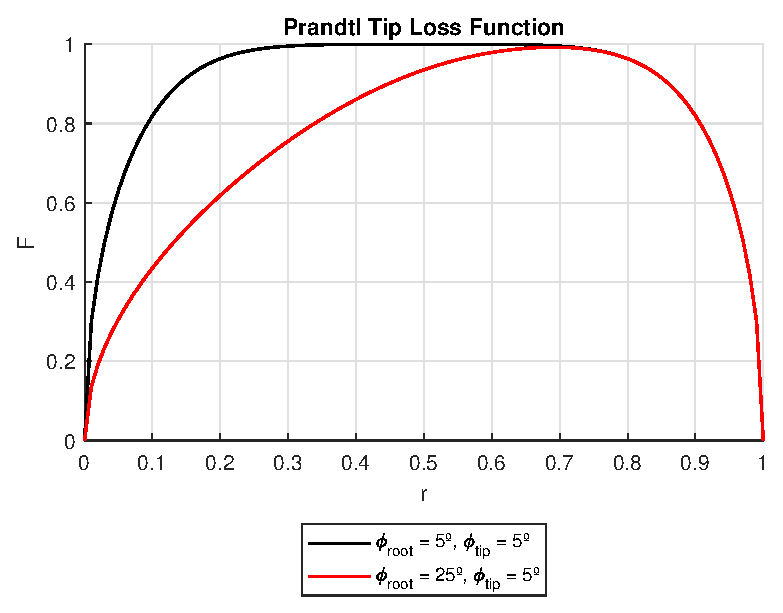
\includegraphics[width=0.5\textwidth]{Figures/background/tiplosses/prandtltiplossfunction.eps}
    \caption{Prandtl Tip Loss Function}
    \label{fig:fullprandtltiplossfunction}
\end{figure}

\textcolor{blue}{analisar os dois casos das perdas de ponta}
